\section{Optimizing Pointwise Convolution}
\label{sec:pwconv}
In this section, we demonstrate the workflow of our dynamic blocking strategy as shown in Figure \ref{fig:pwworkflow} and Algorithm \ref{algo:pwalgo}. 
The whole workflow consists of two stages. 

In the first stage, our approach operates in a top-down fashion. 
We use a 3-level hierarchical partitioning method to decompose the output into three levels of tiles, including block level tiles, warp level tiles and thread level tiles. 
There are two main considerations when decomposing the output. First, how tiles are arranged in its upper level tile, and second, the height and width of each tile with the specified layout.

In the second stage, we calculate the exact height and width of thread level tiles. 
Given the number of output elements in each tile and hardware resources constraints, we iterate over all possible configurations of tile height and width of each level and choose the configuration that maxmize the performance most.

Now we give a detailed description of how each stage works.
\subsection{3-Level Hierarchical Partitioning}
In order to make it easier to understand the workflow of this stage, we first describe two important constant parameters and how we determine their values.

The first parameter is the number of warps in a thread block, denoted as $Warp_{num}$.
In order to determin the warp number, we need to consider: (1) small warp number will decrease the opportunity to hide the memory access latency at the warp level;
(2) large warp number will dcrease the number of thread blocks and may lead to SM underutilization.
Baed on both considerations, we decide to set $Warp_{num}=4$.
In our experiments, this value is good enough to provide a satisfied performance.

%this may not be important as i think
The second parameter is the number of thread blocks that can run concurrently on an SM.
We use two values, 2 and 4, for this parameter, denoted as $Block_{num}=\{2, 4\}$. 
There are two reasons for these choices: 
(1) when $Block_{num}=1$ and $Warp_{num}=4$, there are only 4 warps in an SM. 
As each thread can use up to 256 registers, a thread block can use at most $4*32*256=32768$ registers, which is only half of 65536 registers of an SM.
To avoid wasting hardware resources, we set $Block_{num}>1$; 
(2) when partitioning the output with the configuration of 4 thread blocks per SM, we encounter cases in which 5 or 6 thread blocks are actually running concurrently on an SM. 
This is because in some cases, each thread block requires very few hardware resources and more than 4 thread blocks can run concurrently on one SM.
Therefore, when searching for the best configurations, we only need $Block_{num}=\{2,4\}$.

Now we demonstrate the workflow of our 3-level hierarchical partitioning.
In Figure \ref{fig:pwworkflow}, we show two logical layouts of output, $F_N$ and $I_N \times I_H \times I_W$ represent the filter and input dimensions of the output respectively.
In the first level, we partition the output based on the number of filters, $F_N$.
When $F_N \ge 48$, we choose layout \textbf{\emph{L1}} and distribute filter channels across threads of the same warp. 
Otherwise, we choose layout \textbf{\emph{L2}} and distribute input channels.
The rationale behind this choice can be described as follows. 
The number of filters, $F_N$, is fixed once the structure of a CNN is determined. 
But the dimension of the input will be affected by the batch size, $I_N$, during inference and training.
For the sake of simplicity, we design and implement our dynamic partitioning startegy to utilize layout \textbf{\emph{L1}} whenever there are enough filters to be distributed across threads.
We will explain later in this section why we choose 48 as the boundry of layout \textbf{\emph{L1}} and \textbf{\emph{L2}}.

Next, we partition both layouts of output into block tiles along the filter dimension. 
For the layout \textbf{\emph{L1}}, we halve the filter dimension if $F_N \geq 512$. 
The reason is that if we let each block tile process excessive amount of filters, there will be few options for channel number{\color{red}explain this in previous text} when distributing channels across threads. 
This may cause our dynamic partitioning startegy to find a sub-optimal configuration for pointwise convolution.
For the layout \textbf{\emph{L2}}, we halve the filter dimension if $F_N \geq 24$.
Last, we halve both dimensions of each block tile and generate $2 \times 2$ warp tiles. The height and widht of a warp tile are represented as $Warp_H$ and $Warp_W$ respectively.

\subsection{Distribute Channels Over Threads}
{\color{red}illustrate the max number of filters and inputs a thread can process}
In this stage, we iterate over all candidate combinations of channel count and $Warp_H$, and select the combination that leads to optimial SM utilization and arithmetic intensity.

Now we describe how to determine the candidates for channel count and $Warp_H$ with layout \textbf{\emph{L1}}. Layout \textbf{\emph{L2}} has a similar process.
Assume that we distribute 8 channels ($C_{num}=8$) across 8 threads, which means that 8 threads will load 8 channels of the same filter into registers. 
Therefore, 32 threads of a warp can load 32 channels of $32/8=4$ filters at the same time, we denote this number as $F_{num}=32/C_{num}$.
And then the number of filters each thread needs to process can be calculated with $T_F=Warp_H/F_{num}$.
To fully utilize a warp, the channel count should be a power of 2.
Thus, the condidates for channel count are $C_{num}=\{1,2,4,8,16,32\}$.

Next, we demonstrate how to determine the candidates for $Warp_H$ based on the size of input dimension, $I_N \times I_H \times I_W$.
If the size of input dimension is large, we prefer to choose large $Warp_H$ because using small $Warp_H$ will generate more thread blocks and results in multiple loads of shared filters.
If the size of input dimension is small, we prefer to choose small $Warp_H$ because using large $Warp_H$ will generate a few thread blocks and result in SM underutilization.
Since each thread loads at most 12 input elements, we set the upper limit of large $Warp_H$ to 12 and lower limit to $12/2=6$. 
Therefore, the condidates for large $Warp_H$ are $Warp_H=\{6,7,8,9,10,11,12\}$.
The candidates for small $Warp_H$ are $Warp_H=\{2,3,4,5,6,7,8\}$.
In our experiments, there is no clear boundry between large and small candidate sets of $Warp_H$, therefore we let both sets overlap in the middle values.
The boundry between large and small size of input dimension is experimentally determined as $I_N \times I_H \times I_W=16 \times 14 \times 14$.

When searching for the optimal combinations, we only consider combinations that staisfy hardware constraints, including registers and shared memroy.
Based on $Block_{num}$, we calculate the number of registers each thread can use and the size of shared memory each thread block can use, denoted as $Limit_R=65536/(Block_{num}*4*32)$ and $Limit_S=64*1024B/Block_{num}$ respectively.
Each thread calculates $Warp_H \times T_{num}$ output elements and thus needs $R_O=Warp_H \times T_{num}$, $R_I=Warp_H$ and $R_F=T_{num}$ registers to store output elemnts, input elements and filter elements respectively.
In cases where the computation workload is small, we try to let each thread accumulates $Warp_H*T_{num}$ output elements $k \in \{1,2,3,4\}$ times.
The constraints can be formulated as follows:
\begin{equation}\nonumber
R_{LF}=\frac{C_{num}*k*Block_W}{128},R_{LI}=\frac{C_{num}*k*Block_H}{128}
\end{equation}
\begin{equation}
    \label{fo:limitr}
R_O+R_I+R_F+R_{LF}+R_{LI}+para \leq Limit_R
\end{equation}
\begin{equation}
    \label{fo:limits}
(Block_H+Block_W)*C_{num}*k*4*2 \leq Limit_S
\end{equation}
where $R_{LF}$ and $R_{LI}$ are number of registers used to store filter and input elements loaded from global memroy respectively, $para$ is the number of additioal registers allocated by the compilter. The values of $k$ and $para$ for each kernel are determined through an off-line method. 
\begin{figure*}
	\centering
    %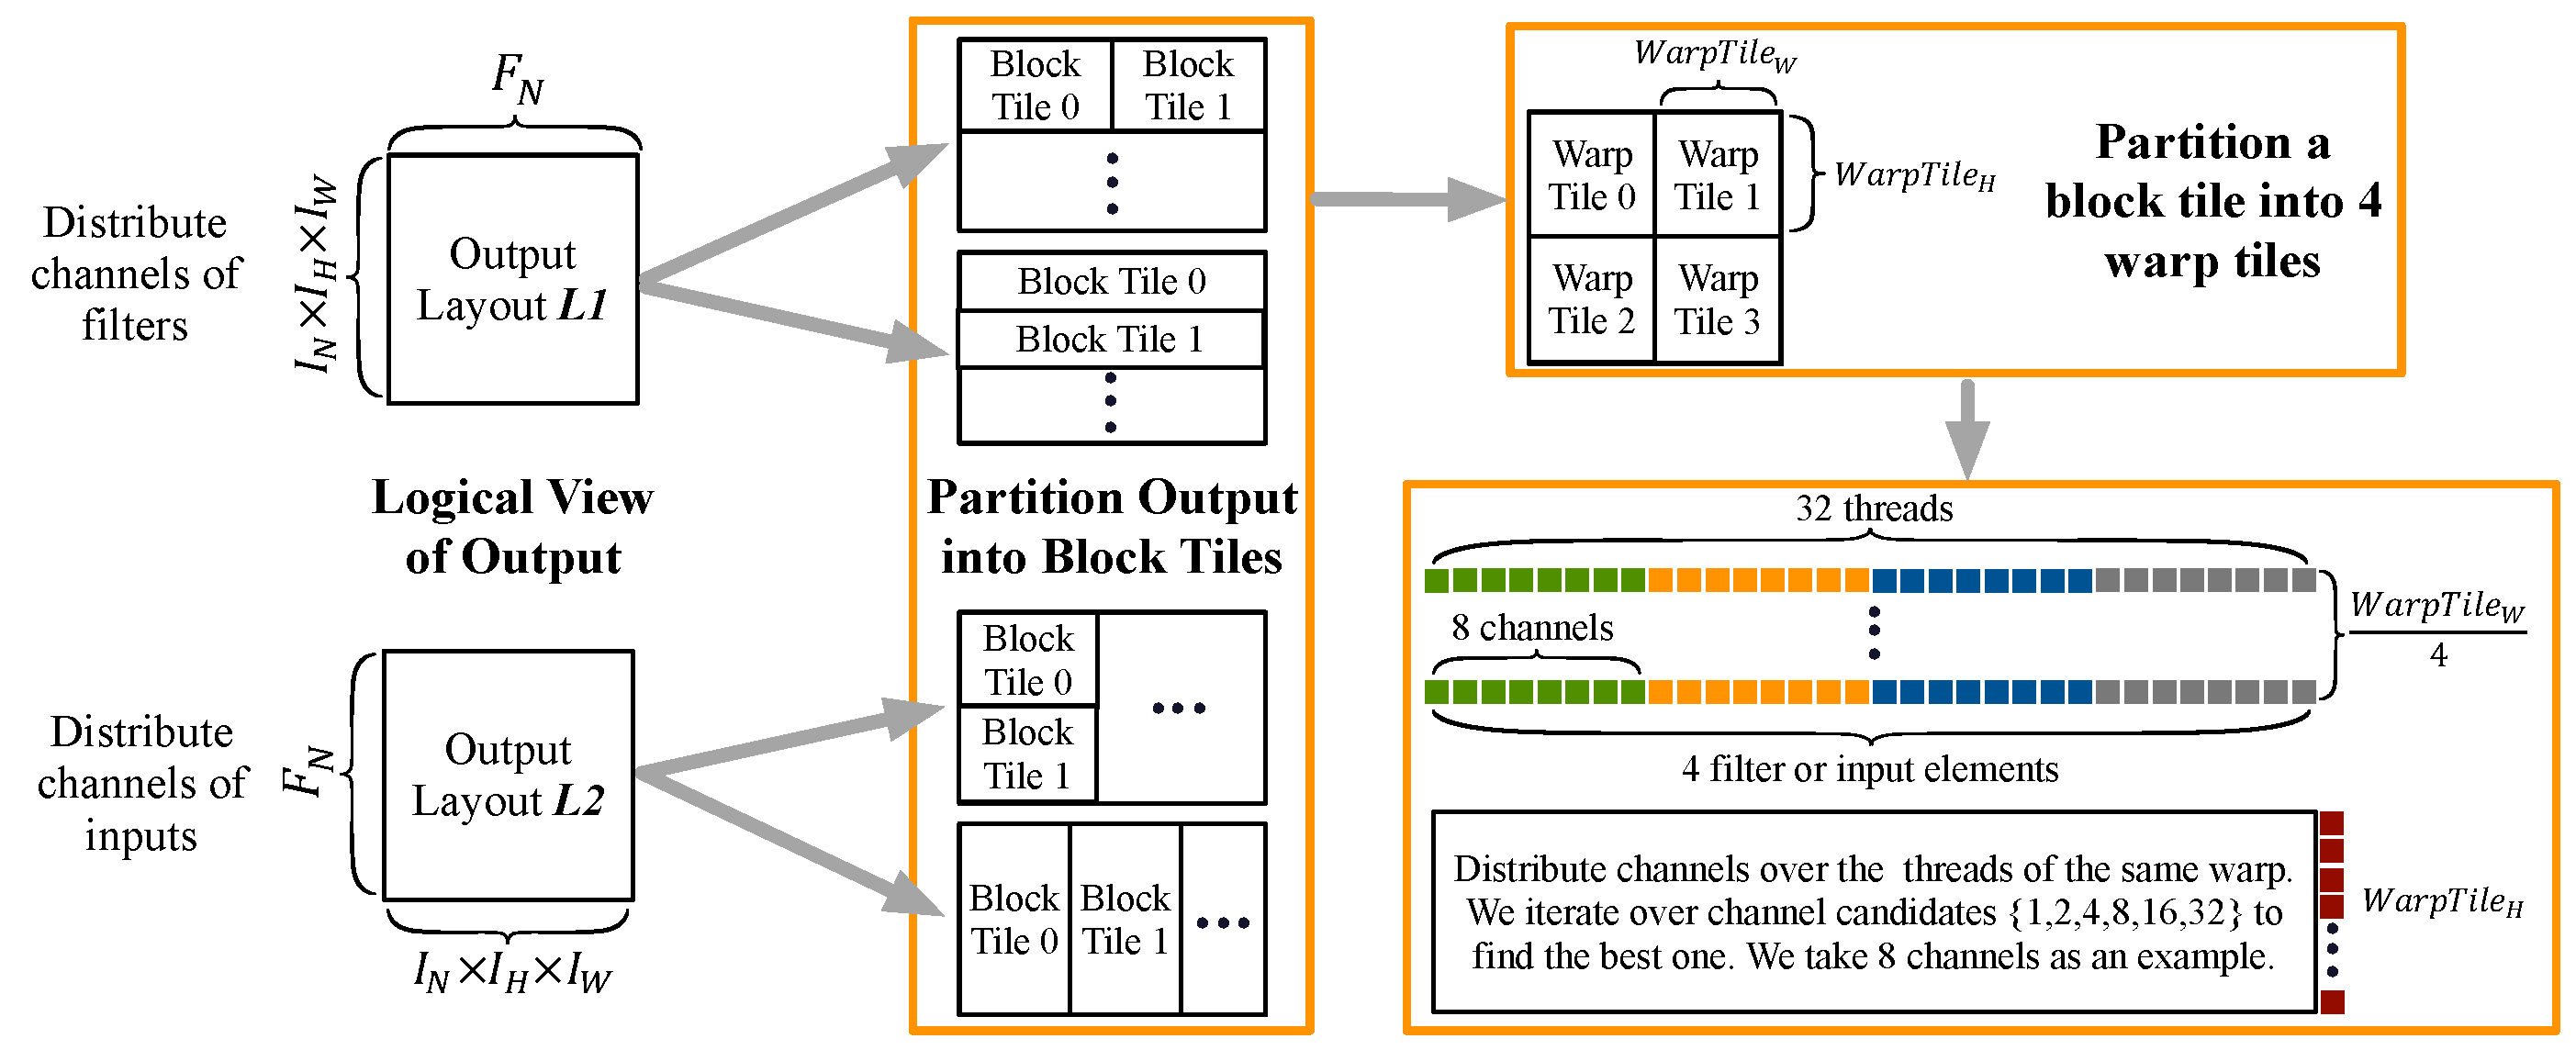
\includegraphics[width=\columnwidth]{./figure/pwworkflow1.eps}
    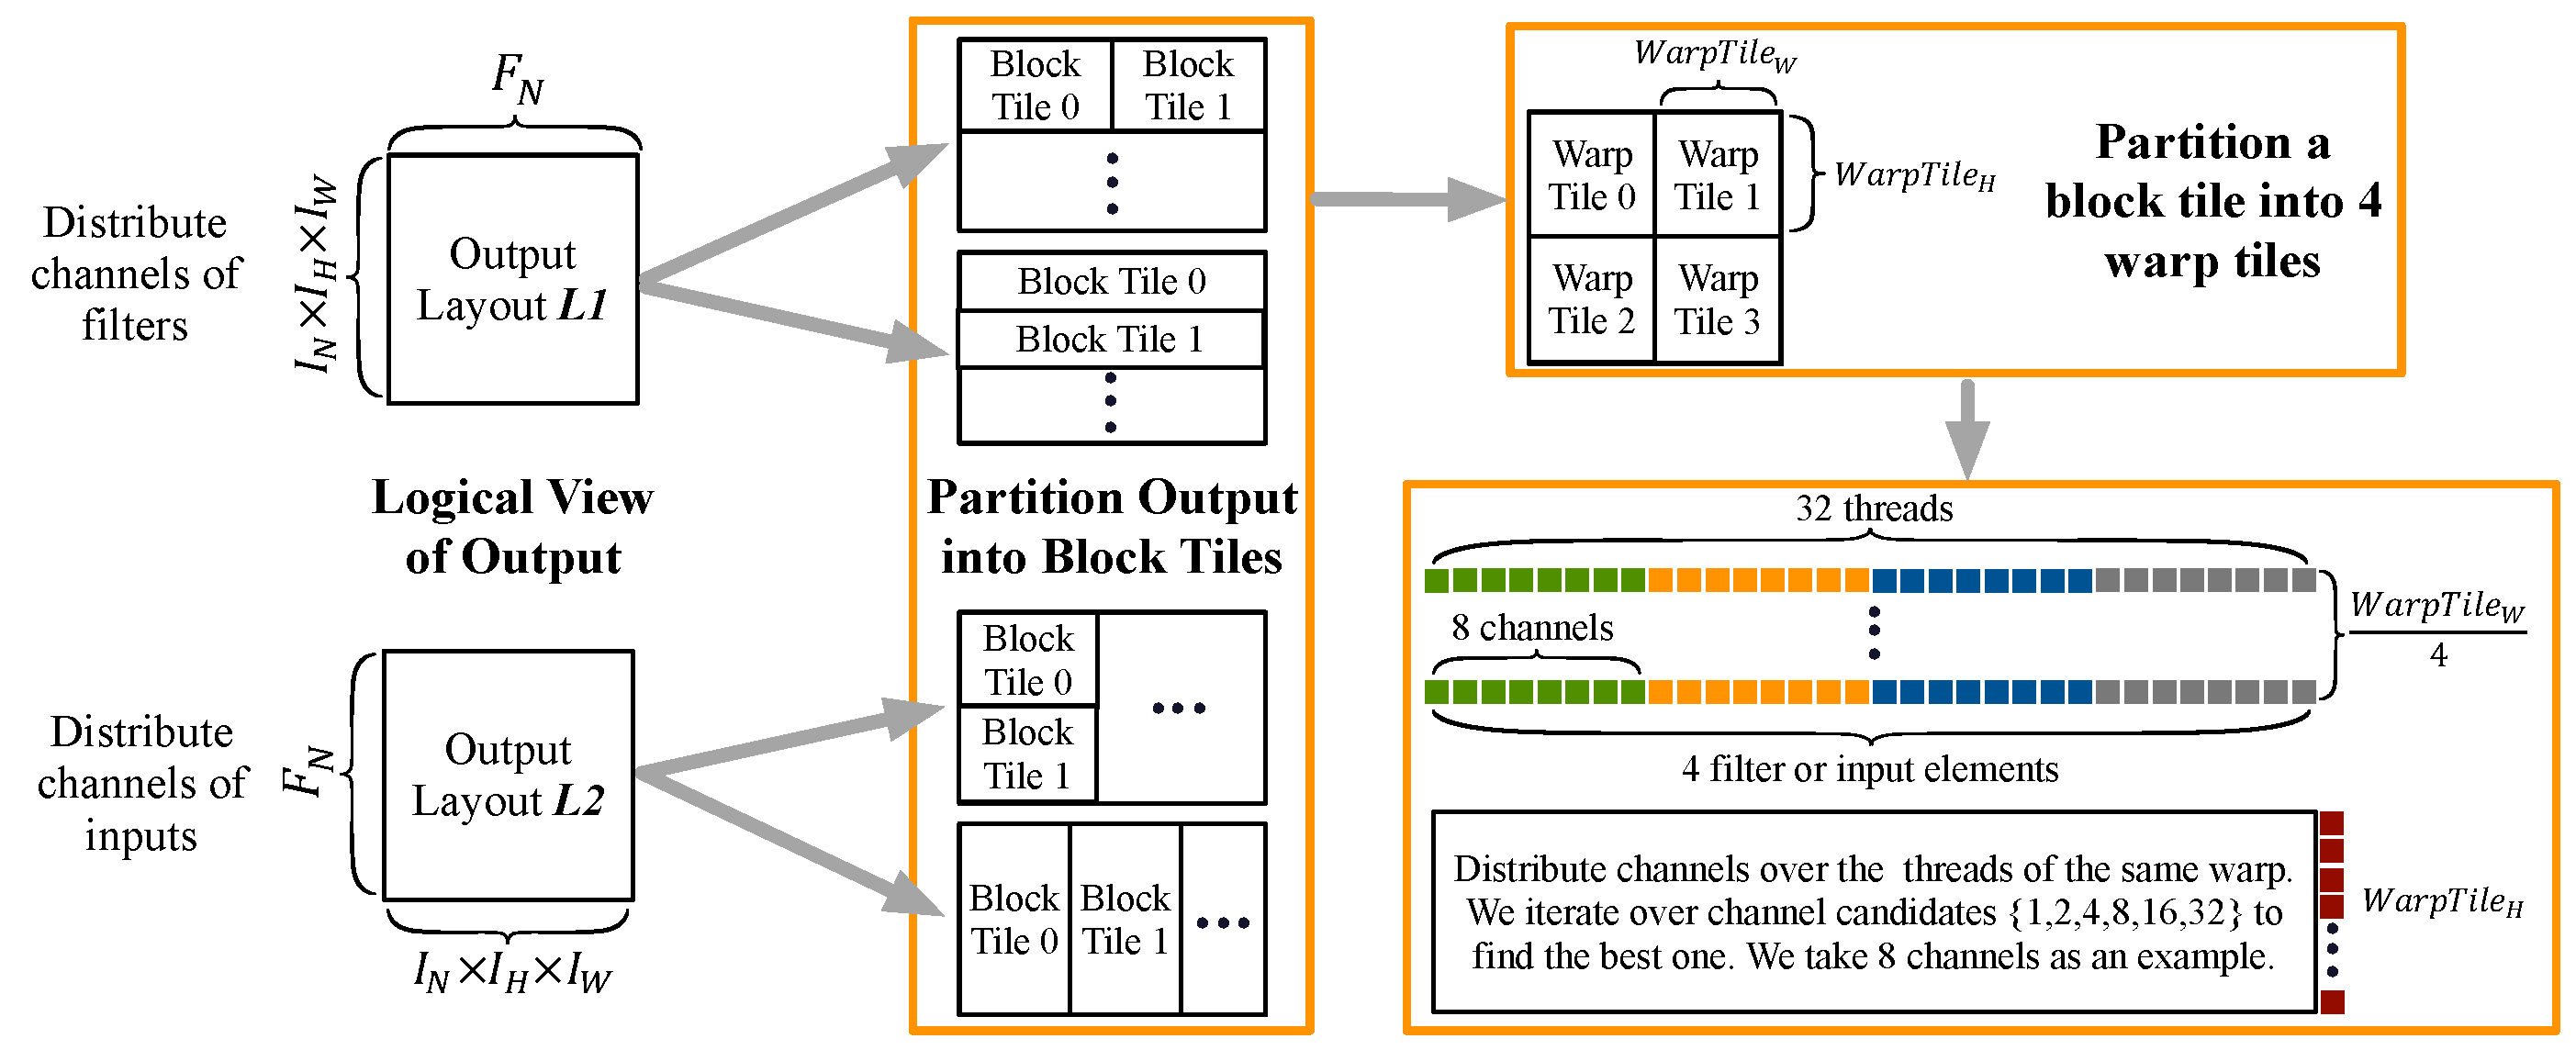
\includegraphics[width=0.95\textwidth,height=7cm]{./figure/pwworkflow1.eps}
    \caption{} \label{fig:pwworkflow}
\end{figure*}
\begin{algorithm}[t!]
    \small
        \KwIn{$I$, $F$}
        \KwOut{$O$}
        Calculate how many output elements one SM needs to process if we want to fully utilize GPU, denoted as $O_{sm}$\;
        \tcp{below codes are executed on CPU}
        \tcp{we have two options for block tile number, one SM contains 2 or 4 block tiles}
        \ForEach{block tile number of one SM}{
            Use $BlockTile_{count}$ to denote the number of block tiles resided on one SM\;
            \ForEach{block layout}{
                Calculate the width of a block tile, denoted as $BlockTile_W$\;
                $BlockTile_H = \frac{O_{sm}}{BlockTile_W * BlockTile_{count}}$\;
                \If{$BlockTile_H > 32$}{
                    $niter = BlockTile_H/32$\;
                    $BlockTile_H = 32$\;
                }
                $WarpTile_H=\frac{BlockTile_H}{2}$\;
                $WarpTile_W=\frac{BlockTile_W}{2}$\;
                \tcp{there are 6 choices for channel count, 1,2,4,8,16,32}
                \ForEach{channel count}{
                    Use $C_{count}$ to denote how many threads are uesed to calculate channels of the same output element.\;
                    $filter_{num} = \frac{32}{C_{count}}$\;
                    $filter_{num} = \frac{WarpTile_W}{filter_{num}}$\;
                    Calculate registers and shared memory usage under this configuration, and evaluate if the usage not exceeds the limit.\;
                    record the configuration with smallest register usage. 
                }
            }
        }
        \tcp{below codes are executed on GPU}
        All threads in a thread block cooperate to load the needed input and filter into shared memory\;
        $\_\_syncthreads()$\;
        \For{$iter \gets 0$ \KwTo $I_C$ By $C_{count}$}{
            load next $C_{count}$ channels for input and filter into registers\;
            load current channels of input and filter into registers\;
            calculate output elements\;
            write registers of next channels into shared memory\;
        }
        use segmented parallel reduce to get the final output elements and write the result to global memory\;
        \caption{Pointwise Convolution Optimization}
        \label{algo:pwalgo}
\end{algorithm}

To guide the search for the optimal combination of $Block_{num}$, $C_{num}$ and $Warp_H$, we use two metrics named SM utilization ($SM_{util}$) and the difference between $Warp_H$ and $T_{num}$ ($D$).
Two metrics can be calculated as follows:
\begin{equation}
    SM_{util}=\frac{F_N}{Block_W}*\frac{I_N*I_H*I_W}{2*Warp_H}
    \label{fo:smutil}
\end{equation}
\begin{equation}
    D = |Warp_H-T_{num}|
    \label{fo:diff}
\end{equation}
We will demonstrate how to select the combinations based on bath metrics in the next section.

\subsection{Putting Togtther}
We first choose the layout of output and partition the output into block tiles based on the number of fitlers ($F_N$) and choose the candidate set for $Warp_H$ based on the size of input dimension ($I_N*I_H*I_W$).
Then we iterate over all combinations of $Block_{num}$, $C_{num}$ and $Warp_H$, and keep the combinations that satisfy the constraints $Limit_R$ (Formula \ref{fo:limitr}) and $Limit_S$ (Formula \ref{fo:limits}).

Next, we calculate values of $SM_{util}$ (Formula \ref{fo:smutil}) for all satisfied combinations and select the optimal combination with following steps:
\begin{enumerate}[Step 1]
    \item If all values of $SM_{util}$ are greater than or equal to 1, we select the combinations that possess the smallest and close to the smallest values.
    The reason is that when $SM_{util}$ is greater than or equal to 1, all SMs are utilized, in which case we want to reduce the number of thread blocks to reduce the number of loads of shared filters or inputs between multiple thread blocks.
    \item If there are values of $SM_{util}$ less than 1, we first collect the combinations that posess this kind of values. Then, among these combinations, we select the combinations that possess the biggest and close to the biggest values.
    The reason is that when $SM_{util}$ is less than 1, there are idle SMs, in which case we want to increase $SM_{util}$ to fully utilize SMs. We do not want $SM_{util}$ to exceed 1 becuase that will incure more memory operations.
    \item Among candidate combinations collected in Step 1 or Step 2, we select the combination with the smallest value of $D$ (Formula \ref{fo:diff}).
    We prefer smaller values of $D$ becusae the values of $Warp_H$ and $T_{num}$ are more close, we can use less memory operations to generate the same amount of output elements.
\end{enumerate}

In stage 3, we choose the pointwise convolution kernel based on the selected combination of $Block_{num}$, $C_{num}$ and $Warp_H$. In this kernel, each thread block first loads channels of corresponding inputs and filters into shared memory. Then, each thread accumulates output elements. Meanwhile, each thread corraporates to load next $k*C_{num}$ channels into another shared memory. And repeat the process until all channles have been accumulated to output elments.
Finally, use a warp level segmented parallel reduction to reduce results in different channels into the final result and write to global memory.  